\chapter{Background and Literature Review}\label{C:ex}
\section{Background}
\subsection{QoS Properties}
Quality of service (QoS) is one of the important factors to consider when composing services. It defines the non-functional requirements of a service, such as response time, execution cost, availability, reliability etc. Good quality of service means achieving certain QoS goals which are termed QoS values or QoS properties. These QoS properties indicate whether a Web service is reliable, trustworthy or efficiency. Their significance stems from the fact that a Web service may be functionally capable of performing a given task, but might not be reliable or efficient enough to achieve users' satisfaction. Web services are usually rated using multiple QoS values, each value representing an aspect, or QoS property, of the Web service. QoS properties are the most commonly used characteristics for measuring the quality of Web services and even composite services, as they indicate whether a service is capable of meeting users' expectations.\par

To model the performance of service compositions we considered four QoS attributes: availability, reliability, execution cost and response time. We chose these because they are commonly used in this field \cite{4,14,15,16}. \par
According to \cite{4,11,18}, the four above-mentioned QoS properties are defined as follows:\par

Execution Cost is the amount of money that a service requester has to pay for using the Web service. The global execution cost of a composite set of services can be treated as the sum of the execution costs of all the operations invoked by the services used. For example, the total execution cost of the composite service in Figure \ref{fig:process} is total execution $C = C(S_{1}) + Cost(S2) + Cost(S3) + Cost(S4)$.$w_{1} + w_{2} + w_{3} + w_{3} = 1$.\par
The response time of a single task is the time which elapses between sending a task request and receiving a response. Web service composition allows services to execute in parallel. Thus, when considering a step where two tasks execute in parallel, the path with the longest response time is chosen to calculate the time taken for that step.\par
For example, in Figure \ref{fig:process}, which shows an example Web service composition, services \emph{S2} and \emph{S3} can be executed in parallel. The response time depends on S2 and S3's local QoS duration property values. If S2's QoS duration property value is greater than S3's QoS duration property value, then the overall response time of the composite service can be computed as the sum of all three service nodes S1, S2 and S4's local QoS duration property values.\par
Availability is defined as the ratio of (1) the time during which a service is ready for use and (2) the time during which the Web service exists. The global availability of a composite Web services can be computed as the product of the local availabilities of the Web services used in the service composition.  For example, the availability of the composite service in Figure 2.1, can be computed as Availability(S1) x Availability(S3) x  Availability(S2) x Availability(S4). \par
Reliability is the how reliable message delivery is to the Web service within the maximum permitted time frame. Global reliability can be calculated as the product of the local reliabilities of the Web services used in the service composition. For example, the reliability of the composite service in Figure 2.1, can be computed as Reliability(S1) x Reliability(S3) x Reliability(S2) x Reliability(S4). \par
\begin{figure}[H]
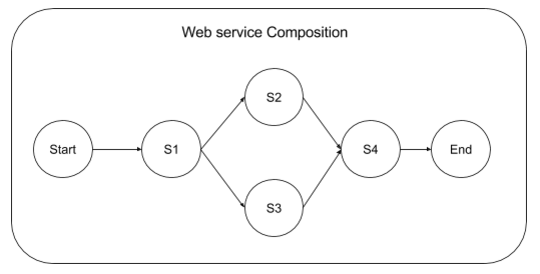
\includegraphics[width=9cm]{Figure2-1ExampleWebServiceComposition.png}
\centering
\caption{Example Web service composition}
\end{figure} 
\subsection{Neo4j graph database}
We employed a Neo4j \cite{6} graph database for our project because it is suitable for representing connected and directed Web services and it allows for very fast retrieval, traversal and navigation of data. A Neo4j Graph Database stores all its data in Nodes and Relationships. All Nodes and Relationships have their own individual properties. And for each data set we need only create a graph database once, after which we can use this database to solve different composition problems. \par

\section{Literature Review}
Over the past few years, Web services have become widely used. A large number of complex applications can be developed using compositions of existing services. Automatic Web service composition technology has become a major focus and challenge in building robust applications which make use of distributed services which provide various functions. Many approaches have been developed for Web service composition, but only a few of them use the concept of graph theory. In this section, we will present a brief overview of some graph-based techniques that deal with automatic Web service composition.\par
Da Silva A. S.et al. presents in \cite{2} an evolutionary computation technique that performs fully automated Web service composition using graph representations for solutions. There are two steps. The first step is to initialise the population by employing a graph building algorithm based on the planning graph approach described in composition literature \cite{3}. The second step is to perform mutation and crossover operations on selected candidates, to generate a new set of candidates and evaluate the fitness of those candidates.\par
The drawback of the approach in \cite{2} is that the graph mutation space contains a lot of invalid service compositions that either violate the constraints of service dependencies or deteriorate the overall performance. Another disadvantage is that the system saves all the Web service dependencies in memory. With every new service request, this approach needs to regenerate all the dependencies again which incurs expensive computation costs. Furthermore, the cost of executing the graph building algorithm is high, since the graph building algorithm is employed twice, in two different processes, namely in the process of generating initial populations and the process of performing mutation and crossover operations.\par
Seyyed, V., H et al. \cite{5} uses a graph search algorithm to construct Web service compositions. This algorithm is based on input-output dependencies of Web services. In order to solve the service composition problem, the authors divide the process into two steps. The first step is to look for Web services which can potentially participate in the composition, and the second step is to find a corresponding composition. The graph building algorithm constructs edges between directly related Web services which have data dependencies between the inputs and outputs of these services. The main shortcoming of this approach is that semantic functions are not considered in the dependencies between input and output parameters. Thus there is no guarantee that a generated composite service will provide the precise functionality requested by the user.\par
The Web service composition approaches proposed by Da Silva A. S.et al. et al. in \cite{2} and Seyyed, V., H et al. in \cite{5}, also share a common drawback. They don't include quality of service in their approach. This means the resulting Web services may not perform tasks that meet a user's non-functional requirements.\par
As we seen above, existing graph-based approaches need to build a data dependency graph for each given task. However, database dependencies between services in a service repository remain stable for all service tasks. Therefore, once a service dependency graph is generated it is best stored and used for all service tasks. In this project we propose to use a graph database to store the information related to services and dependencies of services of a service repository. With each new service task we can utilize existing dependency information contained within graph database dependency graphs. Our approach also takes quality of service (QoS) into consideration by including QoS properties with each edge between Web services.    